Metamaterials are materials with a structure which is smaller then the wavelenght of ligth. The special properties of metamaterials is  based on the fact that they have a negative permeability $\mu$ and permittivity $\epsilon$. That leads to a negative refractive index $n = \sqrt{\epsilon \cdot \mu}$. 
The Lorentz-Oscillator model describes the optical characteristics of intraband  and the Drude model of the interband transitions and both can show  a negative $\epsilon$. The negative $\mu$ can be explained with the Kirchhoff's circuit laws. \\
The reflection spectrum of SRR shows frequency and polarisation dependencies.
\begin{figure}[H]
\centering
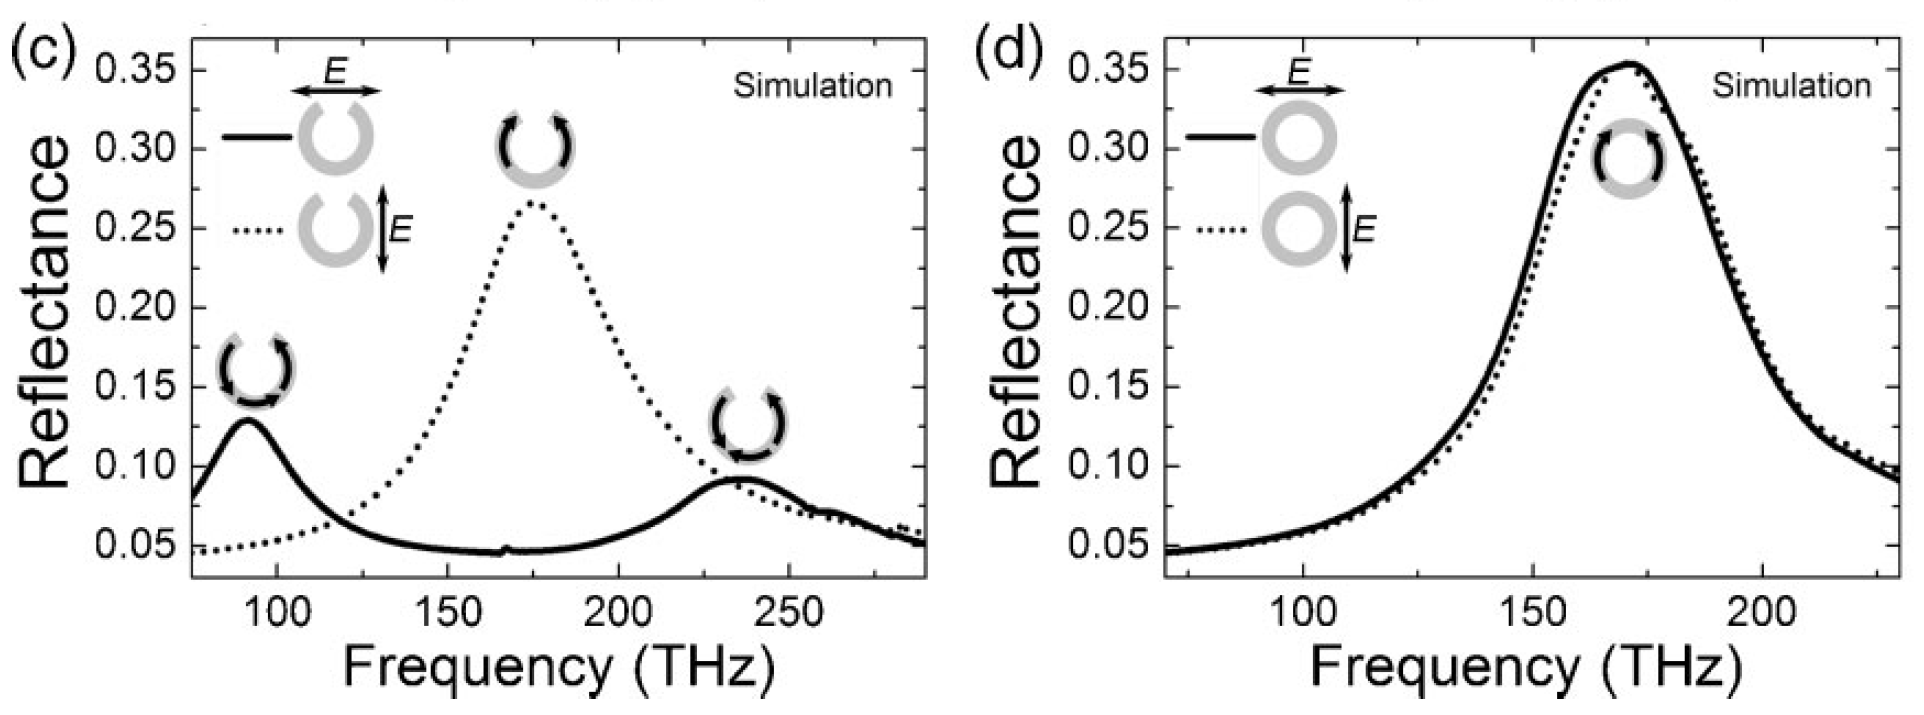
\includegraphics[scale=1]{../figures/spectrum_theory.png}
\caption{Simulated reflection spectrum of a split-ring and a full-ring for different polarisations. \cite{paper_Giessen_meta}  }
    \label{spectrum_theory}
\end{figure}
